\section{Methodology}
%% i.e. Pipeline structure
%%Joe

% Pipeline for processing of GPS traces
%  - filtering of waypoints
%  - map matching using graphhopper
%  - remove matched trips that have an average speed over 120kmh, or a duration less than 1 minute - 9\% of trips removed.
%  - calculate link entry and exit times - simple formula
%  - convert to matsim events
%  - run traces through event processing to calculate externalities
%  	- for emissions cap link average speed at link freespeed 
%  	- road types taken from OSM
%  	- end result is calculation of emissions and delays for each trip leg
In this section, the methodology for imputing externalities on GPS is presented. For the imputation, reference values for air pollutant and congestion production are required. For emissions, the HEBFA database v3.2 is used. 
For congestion, the output of a 10\% sample form the 2015 MATSim scenario for Switzerland (see section \ref{matsim-scenario} is processed to determine average hourly values per link for both the congestion caused by a vehicle on the link, and the delay experienced. 
This is done using the approach of \citet{kaddoura}, described in more detail in section \cite{section:kaddoura_congestion_approach}.

\subsection{GPS processing pipeline}


 A Multistage pipeline has been developed for imputing externalities on GPS traces using the MATSim framework. 
 The pipeline consists of the following steps, described in more detail below. 
 The pipeline can essentially be delineated into two parts, the first creates a series of MATSim events representing the map matched path of the GPS traces. 
 The second processes those events using the reference values mentioned above to impute the generated pollution and delays.

\begin{enumerate}
 	\item Cleaning of GPS data
 	\item Map matching to the MATSim network using Graphhopper
 	\item Calculate link entry and exit times
 	\item Conversion to MATSim events
	\item Imputation of externalities on MATSim events
\end{enumerate}


\paragraph{Data cleaning}
GPS data accuracy can vary considerably, depending on the sensor used, the surrounding environment and even geographical location. 
The data collected as part of the green class project included not just longitude, latitude and time, but also an accuracy inicator, in meters. 
The filtering was performed only using this metric, with any points with an accuracy worse than 200 meters were excluded from the dataset. 
This proved sufficient for effective map matching. Other techniques include exluding points based on the speed between consecutive points. 
It is worth noting that Graphhopper also performs some additoinal filtering, removing points within a measurement error of the previous point, in order to speed up the map matching computation. Inconsistencies in the provided GPS data meant that some trips had unusually high average speeds (due to ping-ponging) or very short trip durations. Therefore, Trips with an average speed over $120 kmh\textsuperscript{-1}$ or less than 1 minute duration were removed. The invalid trips made up 9\% of the dataset. The remaining trips show a nice average speed profile (\ref{fig:avg_speeds}).

\createfigure%
	{Histogram of average speeds of trip legs after step 1 (filtering)}
	{Histogram of average speeds of trip legs after step 1 (filtering)}
    {\label{fig:avg_speeds}}
    {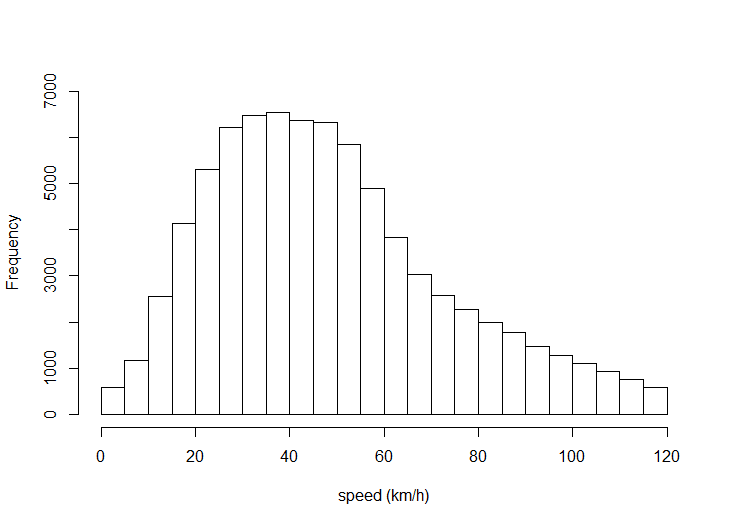
\includegraphics[width=0.7\textwidth]{figures/avg_speed_green_class_matched}}
	{}

\paragraph{Map matching}
Using the MATSim compatible verison of Graphhopper, the GPS points are then matched to the MATSim road network. A measurement sigma of 50m is used to find candidate road segments, and an unlimited distance between consecutive points is allowed. Once the GPS points are matched to road segments, the segment entry and exit times are calculated. This is not performed by Graphhopper. \red{In fact, while relatively state of the art, the Hidden Markov Model approach used by Graphhopper (\cite{vertrbi} doesn't consider speed limits and the respective possible travel times when identifying candidate links for matching.} 

\paragraph{Link entry and exit time calculation}
The map matching module returns a list of $n$ links and the set of GPS points $P(l)$ matched to each link. The recorded time and location of the first and last GPS point $p_{l}$ - ($p_{l,s}$ and $p_{l,e}$ respectively) on each link $l$ are used to estimate the entry and exit times to the link. 
Start and end links must have at least one GPS point associated with them, while intermediate links maybe have none or more GPS points. 
Each GPS point $p_{l,i}$ is projected onto link l, to mark the distance traveled along the link at certain times as $p'_{l,i}$.

A helper function $time\_between(a,b)$ returns the time needed to travel between projected points and verticies of a link. From $p'_{l,e}$ to the end of a link; or the start of a link to the first projected point on a link $p'_{l,s}$. 
$tt(l)$ gives the time needed to travel a link under free flow conditions, and $time_between(p_{l,e}, p_{l',s}$) gives the time difference between the last and first points on two links respectively.

In MATSim the assumptions hold that an agent starts and ends somewhere on a link. Hence, for the first link, only the exit time needs to be calculated, and respectively the entry time for the last link. As such, the algorithm can be separated into two cases:
\begin{itemize}
	\item \textbf{First Link} For the first link $l_1$, $exit\_time(l_1) = time(p'_{l_1,e}) + time\_between(p'_{l_1,e}, l_1)$
%%%	\item \textbf{Last Link} For the last link $l_n$, $entry\_time(l_n) = exit\_time(l_{n-1}) + time\_between(l_{n-1}, p'_{l_n,s})$
	\item \textbf{Other Links} \\
		$entry\_time(l_{j}) = exit\_time(l_{j-1}) $ \\
		\textbf{if} $P(l_j) = \emptyset$ \textbf{then} $exit\_time(l_j) = entry\_time(l_j) + 
										\frac{length(l_j) \cdot time\_between(p'_{l_{j-1},e}, p'_{l_{j+1},s})}{distance(p'_{l_{j-1},e}, p'_{l_{j+1},s})} $ \\
		\textbf{else}  $exit\_time(l_j) = entry\_time(l_j) + time\_between(l_{j}, p'_{l_j,e}) + \frac{time\_between(p'_{l_j,e}, l_{j}) \cdot time\_between(p'_{l_j,e}, p'_{l_{j+1},s})} 
					{time\_between(p'_{l_j,e}, l_{j}) + time\_between(l_{j+1},p'_{l_{j+1},s})}   $ \\
\end{itemize}

\paragraph{Conversion to MATSim events} 
The sequence of links with entry and exit times are then converted to valid MATSim events and grouped by person and date.

\paragraph{Imputation of externalities on MATSim events}
To impute the externalities of each trip leg, The events are processed using a MATSim framework set up with two additional modules. The first, developed by \citet{kaddoura} calculates the pollutant amounts inccured on each link, based on the observed travel speed. Values and emissions factors are taken from the HBEFA database, version 3.2. Average speeds on each link are capped at the link freespeed. The road types for assigning emissions factors are taken from OSM. Each driver is assigned a medium sized vehicle with a 4 cylinder EURO-4 compliant petrol engine. It was not possible at this stage to represent the actual owned vehicles of the study participants.

For congestion, the caused delays per link are imputed from the average hourly values calculated section \ref{avgvalues}. The time lost per link is calculated from the difference between the link travel time and travel time under free flow conditions in the MATSim scenario. From here is it straight forward to determine the total generated pollution and caused and experienced delay per trip leg.
